In Section \ref{sec:research} a case was made for adapting existing repositories to the realities of the current research ecosystem, which is characterised by a highly-distributed architecture; this enables bibliographic metadata to be routinely transferred between the systems that can best fulfil the functions required by the scientific venture, such as dissemination, preservation, discovery, or analysis. Adapting existing systems, instead of building new ones from the ground up is a preferred solution as, most often, software systems encapsulate a high degree of business logic which is undocumented externally and thus, cannot be easily replicated in new solutions. Furthermore, replacing repository solutions entails the migration of records from the old systems to the new ones, and this is generally undesirable as considerable effort needs to be spent in order to ensure the completeness and correctness of the corpus once the migration is completed.

When building new core functionality into existing systems, all parts of the architecture need to be considered in a bottom-top manner. As is the case with most software, in repositories the foundation is represented by the data model which is used to represent bibliographical metadata.

As discussed in Section \ref{sec:data}, the metadata space can be quite complex, both due to the various schemas that can describe its syntax and the various vocabularies prescribing its semantics. Thus, in order to both bring repositories up-do-date with the current ecosystem and also ensure an acceptable degree of viability on the medium and long term, a data model which a high degree of flexibility needs to be built into the core of the system.

\section{The Resource Description Framework (RDF) data model}
\label{sec:rdf}

\gls{rdf} is a model that can satisfy the mentioned requirements; the inception and evolution of \gls{rdf} is interlinked with the one of the \gls{www}, being fundamental in the newer concept of \emph{linked data}\footnote{\url{https://www.w3.org/standards/semanticweb/data}}. Withal, \gls{rdf} is defined as \emph{,,a standard model for data interchange on the Web''}\cite{rdf}. Its capabilities, that allow merging heterogeneous and continually-evolving data with little to no modifications required to the systems managing it, make it a good candidate for handling the complexity mentioned previously. 

At a very high level, \gls{rdf} simply consists of statements about various artefacts, or, to be more in line with the web nomenclature, \emph{resources}. It concerns itself with creating links between disjoint resources, these relationships being called \emph{triples}. 
A triple consists of a subject, a predicate, and an object; for example, in the statement ,,"RDF-Based Workflows for the
Figshare Research Data Repository" is created by Adrian-Tudor P\u{a}nescu'' we have the title of a paper as the
subject, \emph{is created} as the predicate, and the name of the first author as the object. Such triples can be visualised
as directed graphs similar to the one in Fig. \ref{fig:graphinit}.

\begin{figure}[thpb]
  \centering
  % fbox will add a border around the figure
  \fbox{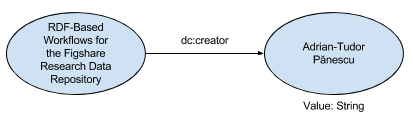
\includegraphics[scale=0.5]{figures/RDF_example.png}}
  \caption{An RDF statement visualised as a directed graph using the \gls{dcmt} vocabulary to name its edge (\emph{dc}: is the prefix identifying this ontology). The subject of this statement should be an \gls{uri}, which would become available after publication in the form of a \gls{doi} for example; for brevity plain character strings were used for both the subject and object}
  \label{fig:graphinit}
\end{figure}

\glspl{uri} are behind one of the main concepts behind \gls{rdf}, resource \emph{identification}. Most frequently, especially in a web context, a \gls{uri} will actually point to a live address from which further information about the resource can be inferred. Nevertheless, this is not a strict requirement, and a \gls{uri} can be unreferenceable; thus, the producers and consumers of \gls{rdf} statements need to agree on the semantics of identifiers. For example, in the graph in Fig. \ref{fig:graphinit}, the \glspl{uri} are marked as pertaining to a well-known vocabulary, namely the \gls{dcmt} ontology; in this way, the consumers of this graph will be able to understand in great detail what is the meaning behind each graph relationship.

Resource identification and \gls{rdf} in general are some of the key technologies in the \emph{Semantic Web}, an extensions of \gls{www} which aims to make the information available on the internet machine-readable, similar in fashion to how the main driver behind the \gls{fair} principles is to make scientific data available to both humans and machines. One way of achieving this with the current infrastructure relates to embedding meta information in web pages in order to improve parsing and categorisation, as the example in Fig. \ref{fig:meta}.

\begin{figure}[thpb]
  \centering
  % fbox will add a border around the figure
  \fbox{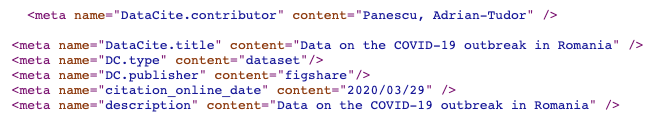
\includegraphics[scale=0.5]{figures/meta.png}}
  \caption{Meta information embedded in the \gls{html} landing page for a dataset published in a repository, allowing systems consuming it, such as web crawlers, to categorise the content with a higher degree of accuracy. The tags are identified using terms from various ontologies, such as \gls{dcmt}, in the same way resources are identified in \gls{rdf}.}
  \label{fig:meta}
\end{figure}

The Semantic Web aims at pushing this even further, by embedding models such as \gls{rdf} in web pages. In this way, the whole content of a single page can be better segmented and annotated, facilitating its consumption by other systems. For example, the title, abstract and other metadata of an article published on a repository can be clearly marked by the serialised\footnote{\gls{rdf} serialisation is discussed in detail further in this chapter.} \gls{rdf} statements that make up the web page. 

Librarianship and repository research has considered the potential of \gls{rdf} and thus employed it for solving various issues in the space. The SciGraph project \cite{scigraph} built an RDF graph starting from Springer Nature journals' and articles' metadata, linked with external information such as institutional affiliations, funding bodies and research grants, citations and references, etc.  In \cite{ichim} the authors describe the model for an \gls{rdf} \emph{federation}, a system in which information from distinct repositories (in this case museum collections) is made available in a consolidated \gls{rdf} format. In \cite{nbdc}, the authors present the experience of building from ground up a life sciences repository in which all datasets are represented as \gls{rdf}; it is interesting to note that, despite the low number of datasets (21), over $45.5$ billion \gls{rdf} triples were generated, demonstrating the inherent complexity of resources, complexity which might be hidden when expressed in natural language. The DSpace repository solution has implemented \gls{rdf} support\cite{dspacerdf}, allowing administrators to convert all held metadata to triples and store them in a specialised store. As mentioned in Section \ref{sec:os}, Fedora Commons has \gls{rdf} deeply embedded in its architecture, in order to ensure that the system can natively communicate and exchange metadata with other systems.

The remaining of this chapter describes how an RDF model can be implemented in an existing data repository system, Figshare, in order to enhance its capabilities of ingesting, administering and disseminating records. This can allow it to support, besides research data, publications, thus achieving the vision of a comprehensive research repository. While this and the previous DSpace example have the same end goal, the solutions are applied to different repository systems\footnote{Moreover, while DSpace is mostly used as an \gls{ir}, Figshare's content mostly comprises of research datasets.} and, more important, have a different approach as to which parts of the software infrastructure are adapted to use \gls{rdf}; for example, due to the data model change, DSpace cannot handle private records when employing \gls{rdf}, while this is not an option for Figshare.

\newpage

\section{From a relational model to RDF in a research repository}
\label{sec:tordf}

Currently, Figshare holds all its metadata in a relational database, with tables and columns for each of the entities required for describing a record. The reasoning behind this choice includes the team's experience with relational systems, the extensive commercial support for such solutions, and the high availability and clustering options provided by these systems even before Figshare's inception. While the current system continues to function well, certain shortcomings were observed when it came to implementing a number of features requested by Figshare's users; the two main requests that triggered the idea of using an RDF-based model are:

\begin{enumerate}
    \item Provide the ability to export metadata in various formats, both predefined in the system and defined ad hoc by end users. Currently, Figshare allows exporting metadata in a fixed set of formats, both in its \gls{oai}-\gls{pmh} interface and web application (see Fig. \ref{fig:figexport}), but this is lacking in both number of formats and the actual metadata which is available when exporting (e.g., almost all options do not contain information about the files pertaining to a record).

    \begin{figure}[thpb]
        \centering
        \fbox{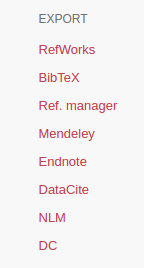
\includegraphics[scale=0.5]{figures/figshare_export.png}}
        \caption{Formats exposed by Figshare for exporting bibliographical information via its web interface.}
        \label{fig:figexport}
    \end{figure}

    \item Provide an easy mechanism for enhancing the main metadata field set. Currently Figshare allows institutional customers to define so-called \emph{custom metadata fields}, which can extend the main set to include information such as, but not limited to, geographical location information, retention dates, or archival markers; the interface for defining such fields is presented in Fig. \ref{fig:caf}. The main limitation of these fields is that they currently cannot be exported in any standard metadata format (e.g., via \gls{oai}-\gls{pmh}) due to their lack of a proper \emph{definition}; for example, when defining a field for holding geographical location information, there is no mean of mentioning that this field follows the definition of the \gls{dcmt} \emph{spatial} one (URI: \nolinkurl{http://dublincore.org/documents/dcmi-terms/#terms-spatial}). This limitation is not only one of the user interface, but also of the application's data model, as the relational scheme is not easy to modify in order to accommodate all the possible definitions and configurations.

    \begin{figure}[thpb]
    \centering
    \fbox{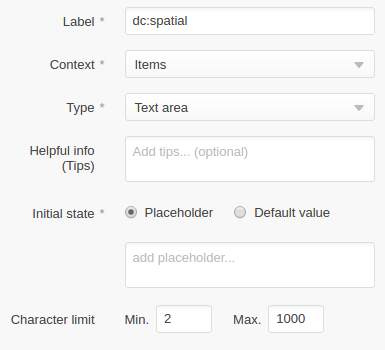
\includegraphics[scale=0.4]{figures/field.png}}
    \caption{Figshare interface that allows institutional clients to define custom metadata fields that can be filled in when creating a new record. Options for defining the type of the value (plain string, date field, etc.), certain validations, and guiding information are included.}
    \label{fig:caf}
\end{figure}

\end{enumerate}

While exploring possible solutions to the issues above it became clear that implementing an \gls{rdf}-based model and workflows would be beneficial not only for answering the two requirements, but also for creating an extensible system upon which various use-cases can build upon.

The first challenge in building an RDF model relates to mapping all of Figshare's metadata fields, defined as columns in the relational model, to a well-defined ontology, vocabulary of terms; this is required in order to be able to properly identify the elements of the triples, as previously explained. In order to achieve this, either an established vocabulary or a custom one can be employed. In general, the first option is preferred as, among other, it avoids the \emph{not invented here} fallacy; moreover, this approach has already been explored by the \emph{figmeta} project\cite{figmeta}, and building upon it can speed up the development of an end-to-end solution.

Figmeta employs the VIVO Core Ontology\footnote{\url{https://wiki.lyrasis.org/display/VIVO/The+core+ontology+and+its+annotations}}. For each column in the relational model, the field in the ontology which is the closest to Figshare's internal
\emph{definition} of the column's contents can chosen; it is worth noting that finding an objective measure of how well this mapping is done is quite difficult as Figshare never provided an exact meaning for each of the columns in the relational model (or metadata fields it expects its records to have). By using these definitions, triples describing a Figshare record can be built, and these can be visualised in a graph such as the one in Fig. \ref{fig:graph}.

\begin{figure}[thpb]
  \centering
  % fbox will add a border around the figure
  \fbox{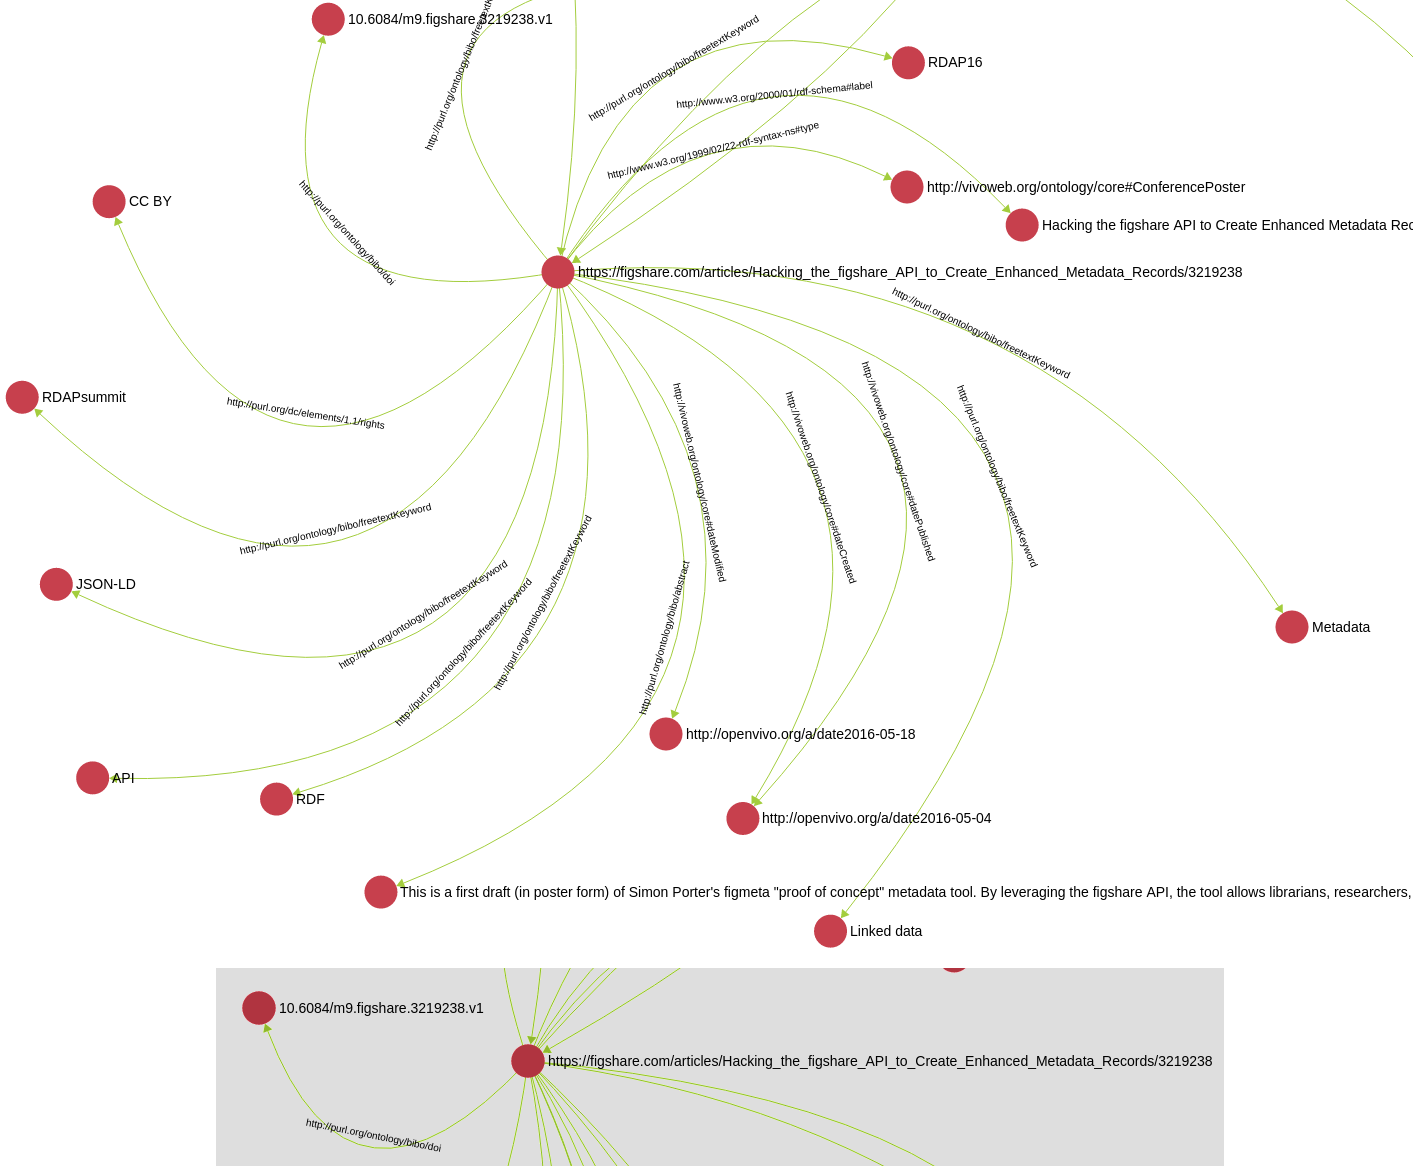
\includegraphics[scale=0.3]{figures/rdf.png}}
  \caption{A Figshare record's RDF graph visualised. Vertices are subjects or objects, while edges are the predicates; edges are always directed from subject to object. The lower snapshot details one of the triples; the predicate is  from the BIBO (\url{http://bibliontology.com/}) ontology, used by VIVO, and associates the subject (a research record) with a \gls{doi}.}
  \label{fig:graph}
\end{figure}

The second challenge relates to the definition of custom, user-defined metadata. While figmeta saved additional fields in a \gls{jsonld} (a  \gls{json} serialisation of RDF triples) data file of the record, another approach which embeds custom defined metadata in the original record
model is proposed here. In order to achieve this, when defining a custom field, apart from the information presented in Fig. \ref{fig:caf}, the user is also requested to specify the ontology in which the field is defined (e.g., gls{dcmt}), and its name in this ontology (e.g., \emph{spatial}). This facilitates the inclusion of this new piece of information in the RDF graph; the predicate is composed of the term name and its ontology (e.g., \nolinkurl{http://dublincore.org/documents/dcmi-terms/#spatial}), and the object os the actual value, specified when the record is created. The subject, in the current configuration, is always the bibliographical record, but due to the flexibility of the RDF model it could become any other vertex in the graph (e.g., one of the attached files, or the author identifier).

Apart from the flexibility, this approach also has the advantage that it considers all metadata fields to be \emph{equal}. In the relational model, where table structure cannot change frequently, the core metadata set is treated as a first-class citizen, while user defined metadata is lacking certain features; for example, Figshare's search system cannot fully query custom medatada fields (e.g., retrieve all records for which \emph{only} the \emph{spatial} field has the value \emph{``Appalachian Mountains''}. The aim here is to devise a uniform representation, where all fields require equal effort in terms of development when a certain functionality is considered.

The third considered challenge relates to the methods used for exporting metadata outside the repository. In the current model, this is done by implementing interfaces between the various aspects of the platform (\gls{oai}-\gls{pmh}, web interface, \gls{rest} \gls{api}) and the relational model; this can become cumbersome, because development time needs to be spent for each new export format, and, even more important, users cannot define their own preferred output.

\gls{rdf} graphs can be serialised in various forms, such as the already mentioned \gls{jsonld}, Turtle or N-Triples; the most popular one, nevertheless, is \gls{rdf}/\gls{xml}, which leverages the adoption of the \gls{xml} format and its ecosystem. As most of the formats currently expected by Figshare's users are \gls{xml}-based, this is a natural starting point; by setting up an \gls{rdf}/\gls{xml} serialisation of the
graph it is straightforward to pivot to any other format by employing \gls{xslt}, a method for transforming \gls{xml} documents to other \gls{xml} representations.

Thus, for example, in order to get a \gls{dcmt} representation of a record modelled using \gls{rdf}, two steps need to be performed:

\begin{enumerate}
    \item Distil a \gls{rdf}/\gls{xml} serialization of the graph. Most \gls{rdf} tools nowadays already include the means for this transformation, and thus, the development effort for this can be delegated to them.
    \item Perform an \gls{xslt} operation from the \gls{rdf}/\gls{xml} document to the \gls{dcmt} one; in order to do this a stylesheet as the one in Listing \ref{lst:xslt} can be employed. Tools for performing the actual transformation are also wide-spread.

\lstinputlisting[language=XML,
                 frame=tblr,
                 captionpos=b,
                 showspaces=false,
                 showstringspaces=false,
                 showtabs=false,
                 stepnumber=2,
                 numbersep=4pt,
                 basicstyle=\fontsize{8}{7}\ttfamily,
                 caption=Example XSL transformation for converting a RDF/XML document to Dublin Core Metadata Terms XML one.,
                 label=lst:xslt]
  {figures/xslt.xml}

\end{enumerate}

An important advantage of this approach is that, starting from the provided \gls{rdf}/\gls{xml} serialisation, users can define their own transformations. This offloads the development work and provides greater flexibility in terms of metadata output. The system also provides a solid
base for developing other internal features; for example, Fig. \ref{fig:tind_search} presents the way in which the Invenio digital library platform can output search results using the \gls{mods}\footnote{\url{http://www.loc.gov/standards/mods/}} schema; as this is also \gls{xml}-based format, implementing the same functionality could be easily achieved via \gls{xslt} applied to \gls{rdf}/\gls{xml}.

\begin{figure*}[t]
  \centering
  % fbox will add a border around the figure
  \fbox{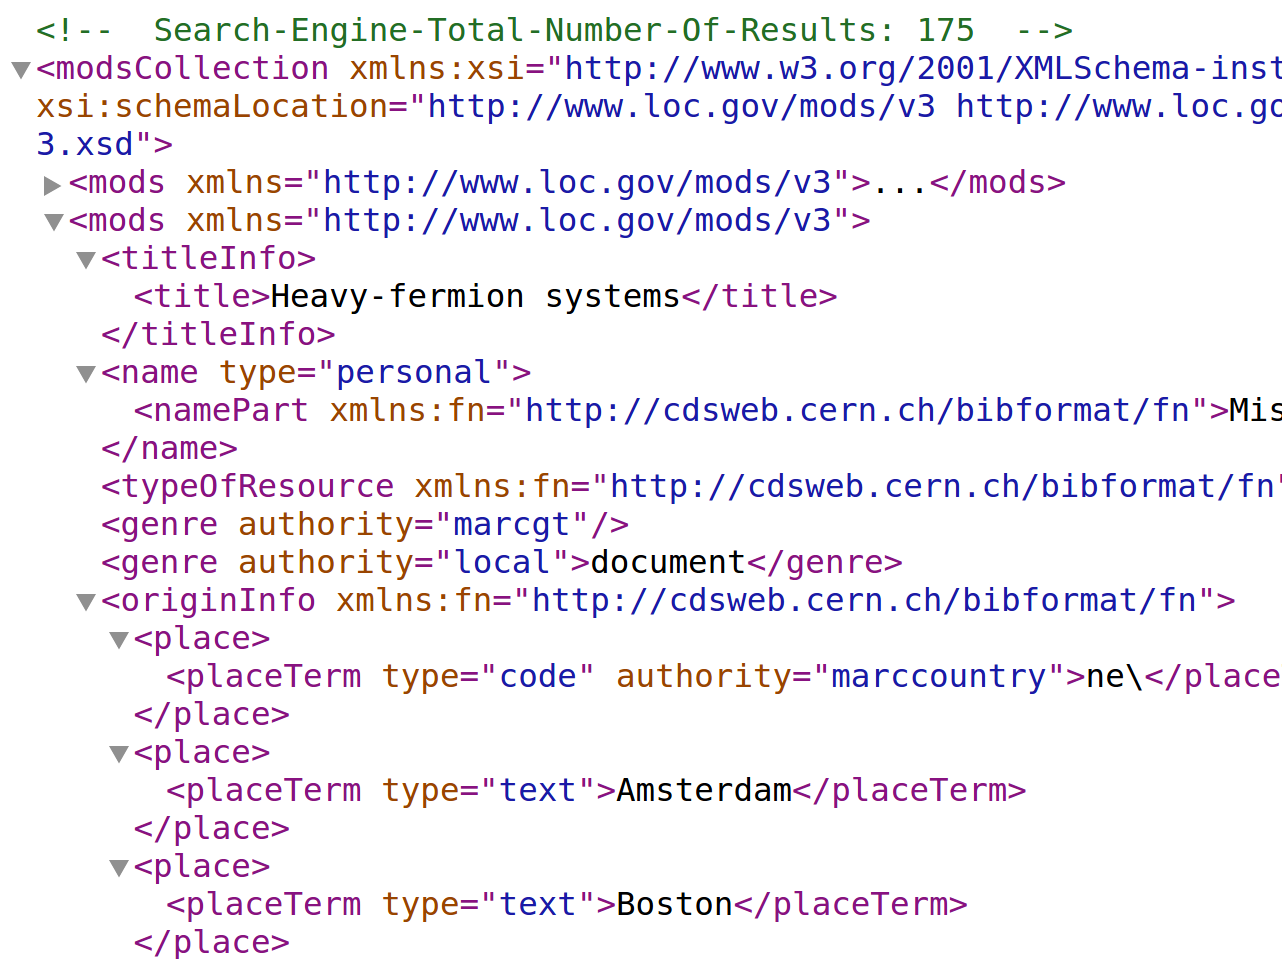
\includegraphics[scale=0.311]{figures/tind.png}}
  \caption{Search results in \gls{mods} format as returned by the California Institute of Technology Library Catalog (\url{https://caltech.tind.io/?ln=en}), a solution based on the Invenio framework.}
  \label{fig:tind_search}
\end{figure*}

Nevertheless, the system does not need to be limited to an \gls{rdf}/\gls{xml} representation; \gls{jsonld} becomes more popular nowadays, especially due to the predominance of the \gls{json} format across web applications, and \gls{rdfa} also starts being used by search engines for achieving a better understanding of the indexed web pages\cite{googleld}.

It is important to note that in order to ease the transition from the relational to the new \gls{rdf}-based data model, the two metadata stores can run in parallel, the RDF system replicating the information in the relational detabase. Moreover, the existing database can continue to function even after the transition is completed, in order to support certain business logic, which better fits the relational model or for which a transition to \gls{rdf} is not fully justified (e.g., account management system). As discussed previously, Fighsare cannot drop support for private records, as the DSpace \gls{rdf} implementation required\cite{dspacerdf}, and such logic can continue to be based on the relational model; similarly, Fedora Commons, which already supports complex \gls{rdf}-based features, continues to use a relational database for persistence. In this manner, a \emph{proof-of-concept}  was developed, outside of the existing data store, in order to demonstrate both the workflows described above the feasibility of the transition strategy\footnote{Proof-of-concept published as \texttt{DOI:}10.6084/m9.figshare.4880567}. 

A final point to consider in terms of implementation relates to the physical storage of \gls{rdf} triples. Solutions include native \emph{triple-stores}, such as Apache Jena\footnote{\url{https://jena.apache.org/}}, graph databases, such as Neo4j\footnote{\url{https://neo4j.com/}}, or relational or document databases that can hold \gls{rdf} serialisations; for example, MariaDB, the relational database used by Figshare, implements a \gls{json} data type\cite{mariadb}.